\documentclass[tikz]{standalone}
%\usepackage[dvipdfm]{geometry}

%graphics

\usetikzlibrary{shapes.geometric, shapes.multipart, arrows, calc, through,intersections}


\tikzset{
    pics/mig/.style = {
        code = {%
        \coordinate (-center) at (0, 0);
        \coordinate (-north) at (0, .5cm);
        \coordinate (-south) at (0,-.5cm);
        \coordinate (-se) at (310:.5cm);
        \coordinate (-sw) at (230:.5cm);
        \draw[line width=1mm](0,0)circle[radius=.5cm];
        }
    },
}
\begin{document}

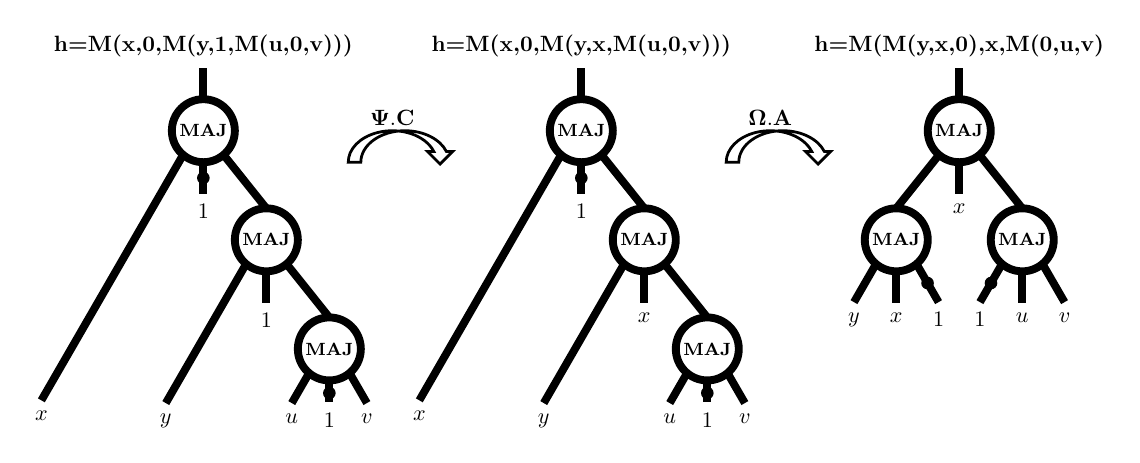
\begin{tikzpicture}[scale=0.8,transform shape,line width=1mm]

\begin{scope}[xshift=-6cm]
\pic(m1) at (0,0) {mig};
\node at(m1-center){\textbf{\footnotesize MAJ}};
\pic(m2) at (300:2) {mig};
\node at(m2-center){\textbf{\footnotesize MAJ}};
\pic(m3) at (300:4) {mig};
\node at(m3-center){\textbf{\footnotesize MAJ}};

\draw(m1-north)-- ++(0,.5)node[above]{\textbf{h=M(x,0,M(y,1,M(u,0,v)))}};
\draw(m1-south)-- ++(0,-.5) node[below]{\textbf{$1$}};
\fill ($(m1-south)+(0,-0.25)$) circle[radius=1mm];
\draw(m1-sw) -- ++(240:4.5)node[below]{\textbf{$x$}};
\draw(m1-se) -- (m2-north);

\draw(m2-south)-- ++(0,-.5cm) node[below]{\textbf{$1$}};
\draw(m2-sw) -- ++(240:2.55)node[below]{\textbf{$y$}};
\draw(m2-se) -- (m3-north);

\draw(m3-south)-- ++(0,-.35) node[below]{\textbf{$1$}};
\fill ($(m3-south)+(0,-0.2)$) circle[radius=1mm];
\draw(m3-sw) -- ++(240:.55)node[below]{\textbf{$u$}};
\draw(m3-se) -- ++(300:.55)node[below]{\textbf{$v$}};
\end{scope}

\begin{scope}[xshift=-3.5cm,yshift=-0.5cm,line width=1pt]
\draw(0,0)arc[start angle=180,delta angle=-160, x radius=7mm, y radius=5mm] -- ++(1mm,0) -- ++(-2mm,-2mm) -- ++(-2mm,2mm) -- ++(1mm,0) arc[start angle=20,delta angle=160, x radius=7mm, y radius=5mm] -- cycle;
\node at (5mm,7mm) {$\mathbf{\Psi.C}$};
\end{scope}

\begin{scope}
\pic(m1) at (0,0) {mig};
\node at(m1-center){\textbf{\footnotesize MAJ}};
\pic(m2) at (300:2) {mig};
\node at(m2-center){\textbf{\footnotesize MAJ}};
\pic(m3) at (300:4) {mig};
\node at(m3-center){\textbf{\footnotesize MAJ}};

\draw(m1-north)-- ++(0,.5)node[above]{\textbf{h=M(x,0,M(y,x,M(u,0,v)))}};
\draw(m1-south)-- ++(0,-.5) node[below]{\textbf{$1$}};
\fill ($(m1-south)+(0,-0.25)$) circle[radius=1mm];
\draw(m1-sw) -- ++(240:4.5)node[below]{\textbf{$x$}};
\draw(m1-se) -- (m2-north);

\draw(m2-south)-- ++(0,-.5cm) node[below]{\textbf{$x$}};
\draw(m2-sw) -- ++(240:2.55)node[below]{\textbf{$y$}};
\draw(m2-se) -- (m3-north);

\draw(m3-south)-- ++(0,-.35) node[below]{\textbf{$1$}};
\fill ($(m3-south)+(0,-0.2)$) circle[radius=1mm];
\draw(m3-sw) -- ++(240:.55)node[below]{\textbf{$u$}};
\draw(m3-se) -- ++(300:.55)node[below]{\textbf{$v$}};
\end{scope}

\begin{scope}[xshift=2.5cm,yshift=-0.5cm,line width=1pt]
\draw(0,0)arc[start angle=180,delta angle=-160, x radius=7mm, y radius=5mm] -- ++(1mm,0) -- ++(-2mm,-2mm) -- ++(-2mm,2mm) -- ++(1mm,0) arc[start angle=20,delta angle=160, x radius=7mm, y radius=5mm] -- cycle;
\node at (5mm,7mm) {$\mathbf{\Omega.A}$};
\end{scope}

\begin{scope}[xshift=6cm]
\pic(m1) at (0,0) {mig};
\node at(m1-center){\textbf{\footnotesize MAJ}};
\pic(m2) at (240:2) {mig};
\node at(m2-center){\textbf{\footnotesize MAJ}};
\pic(m3) at (300:2) {mig};
\node at(m3-center){\textbf{\footnotesize MAJ}};

\draw(m1-north)-- ++(0,.5cm) node[above]{\textbf{h=M(M(y,x,0),x,M(0,u,v)}};
\draw(m1-south)-- ++(0,-.5cm) node[below]{\textbf{$x$}};
\draw(m1-sw) -- (m2-north);
\draw(m1-se) -- (m3-north);

\draw(m2-sw) -- ++(240:0.7)node[below]{\textbf{$y$}};
\draw(m2-south)-- ++(0,-.5cm)node[below]{\textbf{$x$}};
\draw(m2-se) -- ++(300:0.7)node[below]{\textbf{$1$}};
\fill ($(m2-se)+(300:0.35)$) circle[radius=1mm];

\draw(m3-sw) -- ++(240:0.7)node[below]{\textbf{$1$}};
\fill ($(m3-sw)+(240:0.35)$) circle[radius=1mm];
\draw(m3-south)-- ++(0,-.5cm)node[below]{\textbf{$u$}};
\draw(m3-se) -- ++(300:0.7)node[below]{\textbf{$v$}};
\end{scope}

\end{tikzpicture}

\end{document}
